\section{Ejercicio 4: Metaheurística}

  % \begin{figure}[ht]
  %   \begin{center}
  %     \includegraphics[width=0.5\columnwidth]{imagenes/pacman.png}
  %     \caption{Perdidos y con poca fuerza}
  %   \end{center}
  % \end{figure}

    % 1. Describir detalladamente el problema a resolver dando ejemplos del mismo y sus soluciones.
    \subsection{Descripción del problema y solución propuesta}
        En este punto, se pidió realizar un algoritmo basado en una metaheurística que resuelva el problema en cuestión. El mismo al tratarse de una metaheurística puede no dar la solución óptima, y puede no devolver una solución aunque la misma exista.

    % 2. Explicar de forma clara, sencilla, estructurada y concisa, las ideas desarrolladas para la resolución del problema. Utilizar pseudocódigo y lenguaje coloquial (no código fuente). Justificar por qué el procedimiento resuelve efectivamente el problema.
        Se decidió utilizar como metaheurística para resolver esta variante del TSP, GRASP. De esta forma se explora el espacio de soluciones, partiendo de diferentes instancias y tratando de mejorarlas mediante búsqueda local. La idea de GRASP es que cada búsqueda va a converger en caso de ser posible a un mínimo local. Como se comienza de distintas instancias se van a explorar varios mínimos locales distintos, con lo cual la solución se puede obtener tomando la mejor de estas buenas soluciones. Como la eficacia de GRASP depende de empezar de soluciones lo suficientemente diferentes utiliza una heurística greedy a la que le suma aleatoridad, en la cual en vez de seleccionar siempre al mejor candidato para una solución, selecciona uno al azar de un grupo de candidatos (el RCL), cuyo tamaño o criterio de selección es configurable. La otra parte configurable de GRASP es la determinación de cuánto se va a buscar, es decir, cuanto tiempo se va a invertir en generar soluciones greedy aleatoria y tratar de mejorarlas. Para este caso particular de este problema, la implementación de GRASP elegida consiste en lo siguiente: se obtiene una solución (en caso de ser posible) mediante una heurística greedy. La misma es similar a la desarrollada en el ejercicio 2. La diferencia es que se le agrega aleatoridad, ya que no se toma a la estación más cercana sino que se eligen k estaciones más cercanas (siendo k un parámetro configurable) y se elige una al azar de esas estaciones. La misma estación elegida tiene que ser factible de ser visitada. En caso contrario, el algoritmo devuelve que no encontró solución. Si se toma como parámetro k = 1, este algoritmo greedy es exactamente igual al desarrollado en el ejercicio 2 ya que en todas las iteraciones va a elegir al más cercano. Si se toma como k la cantidad de estaciones total, el algoritmo se transforma en uno completamente aleatorio ya que en cada iteración se toma cualquiera estación. Luego de obtenerse una solución a la misma se le aplica la búsqueda local desarrollada en el ejercicio 3 para tratar de mejorarla. Este procedimiento se repite varias veces hasta que se cumple la condición de parada (parámetro configurable). Se usaron dos condiciones de parada distintas: una es determinar una cantidad de repeticiones que se desea realizar el procedimiento (condición sobre la cantidad de repeticiones del ciclo) y la otra es una cantidad de repeticiones en la cual no se mejoró una solución (condición sobre la cantidad de repeticiones sin mejorar). En ambos casos siempre el algoritmo termina ya que en el primer caso se fija la cantidad de repeticiones (por lo tanto el ciclo corre un número finito de veces) y en el otro aunque se elija un número muy grande, siempre a partir de un momento la solución no se va a poder mejorar (cuando se encuentra la óptima), por lo que en el peor caso si la óptima es encontrada rápidamente por el algoritmo, se va ejecutar una vez encontrada, la cantidad de iteraciones fijada, ya que no se va a poder encontrar ninguna mejor. En cada paso, se va guardando la solución mejor que se encuentra. Es decir, se mantiene una solución, que se actualiza en caso de que se encuentre una mejor en cada iteración de este procedimiento. Al finalizar se retorna la mejor solución encontrada.

        El algoritmo propuesto es el siguiente:

         \begin{codesnippet}
            \begin{verbatim}
			enum crit = { A, B }
			
solverEj4(vector<Estacion> estaciones, vector<vector<double> > distancias, n, m,
          k, grasp, crit criterioTipo, int criterioCant, bool vecindarioBusqLocal) {
    solucion s1
    solucion s2
    solucion best
    i = 0
    bool mejor
    double nuevaSol

    mientras (i < criterioCant)
        s1 = greedyRandomized(estaciones, distancias, n, m, k, grasp)
        s2 = solucionEj3(s1, estaciones, distancias, k, vecindarioBusqLocal)

        mejor = False
        nuevaSol = s2.first
        si i == 0 || (nuevaSol > -1 && nuevaSol < best.first) 
            best = s2
            si i > 0
                mejor = True
            fin si
        fin si
          

        si criterioTipo == A
            i++
        fin si

        si criterioTipo == B && mejor == False
            i++
        fin si
		
    fin mientras
    
    devolver best
            \end{verbatim}
            \end{codesnippet}


        El algoritmo consiste en un ciclo, el cual se ejecuta mientras no se haya llegado a la condición de terminación. La condición de terminación está dada por una tupla (denominada criterio) que contiene en su primer coordenada un entero, que es el que se usa en la condición del ciclo para saber si hay que cortar o no. La segunda coordenada es un booleano y sirve para identificar cual de los dos criterios que definimos se está utilizando. El booleano si es verdadero indica que se usa el criterio de parar cuando no se pudo mejorar en k veces la solución siendo k el entero de la primera coordenada. Si es falso, significa que se usa el criterio de correr directamente k veces el ciclo, siendo k también el entero de la primer coordenada.
        En el cuerpo del ciclo lo que se realiza es obtener una solución llamando a la función \textit{greedyRandomized}, la cual realiza lo mismo que la implementada en el ejercicio 2, salvo que en vez de seleccionar a la estación más cercana a la que se puede ir en cada paso, selecciona una al azar de n estaciones cercanas, siendo n el entero \textit{grasp} que se le pasa a la función. Luego de eso se aplica búsqueda local, llamando a la función \textit{solucionEj3}, la cual es exactamente la misma que la desarrollada en el ejercicio 3. Si nos encontramos en la primera iteración del ciclo o la solución obtenida es mejor que la anterior que teniamos, entonces se actualiza la nueva mejor solución obtenida con la encontrada en esta iteración.
        Finalmente se pregunta si se está usando el criterio de ejecutar k veces fijo (con lo cual la variable \textit{criterio.second} sería falsa) y en caso de ser así se suma uno al contador del ciclo. Sino, se trata del otro criterio y sólo se actualiza el contador si no se encontró una mejor solución en la iteración (hecho representado por el valor de la variable booleana \textit{mejor}), sumándole 1.
        Una vez terminado el ciclo se devuelve la mejor solución obtenida.

  \subsection{Experimentación}

    Para poder comparar cada configuración posible y obtener de ahí la configuración óptima, se generaron 30 instancias random, las cuales nos aseguramos que tengan solución. Luego se realizaron dos experimentos. En el primero, se iteró sobre la cantidad de vértices que entran en la RCL. Mientras que en el segundo, se iteró sobre el límite de cada criterio de parada. Para ambos al igual que en el \textbf{Ejercicio 3}, se buscó comparar por un lado, qué configuración devolvía mejores distancias, y por otro qué configuración corría en menos tiempo. En cada gráfico se usaron las siguientes referencias, P = Criterio de paradas, i = Iteraciones del criterio, V = vecindario de búsqueda local, RCL = K vértices que accederan a la RCL.

\subsubsection{Experimento 1: RCL}

En el siguiente experimento, se crearon 30 instancias random. Las mismas tenían entre 1 y 15 gimnasios. Los mismos requerían entre 0 y 20 pociones. Las posiciones de las estaciones también fueron random. Además, estas 30 instancias se copiaron 4 veces, cada una con una configuración distinta. En cada una de las 4 configuraciones se modificó por un lado el vecindario utilizado en la Búsqueda Local y por otro, el criterio de parada en el cual la cantidad de iteraciones del criterio se fijó en 15.

De esta manera las siguientes 4 configuraciones son 

\begin{table}[H]
\centering
\begin{tabular}{ |c|c|c| } 
 \hline
 Instancias&Busqueda Local&Criterio de parada\\ 
 \hline
 Configuración 0 & Vecindario A & Iterar K veces\\
 \hline
 Configuración 1 & Vecindario A & Iterar hasta K peores\\
 \hline
 Configuración 2 & Vecindario B & Iterar K veces \\
 \hline
 Configuración 3 & Vecindario B & Iterar hasta K peores\\
 \hline
\end{tabular}
\caption{Configuraciones experimento 1}
\end{table}


Luego por cada instancia, con cada configuración, se iteró el K de RCL, de 1 a 15. Por cada K, se corrió 20 veces el mismo algoritmo, y se sacó un promedio del tiempo y de la distancia.
Además, se sacó un promedio de la distancia y el tiempo entre las 30 instancias con la misma configuración y el mismo K. De esta manera se contaba con un solo promedio de tiempo y distancia por cada K, y por cada configuracion.

  \begin{figure}[H]
      \begin{center}
        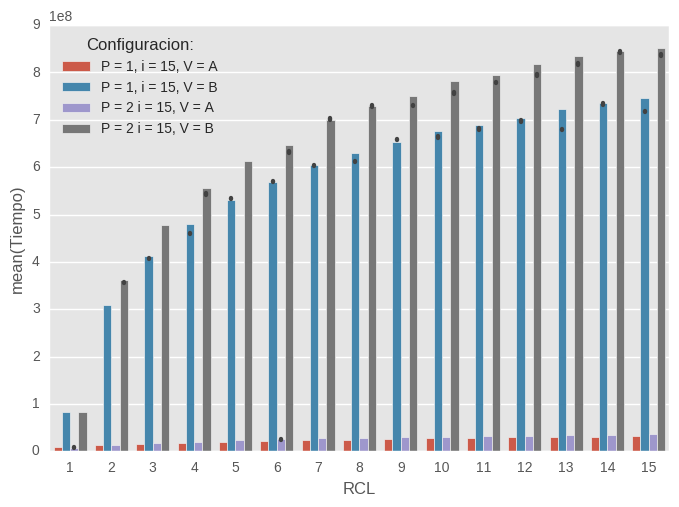
\includegraphics[width=0.7\columnwidth]{imagenes/Ej4/ej4_exp1_Tiempo.png}
      \end{center}
  \end{figure}


  Luego, a partir de esta experimentación, dado que a medida que crecía la lista RCL, crecía la cantidad de elementos a randomizar, pudimos observar cómo esto impactaba directamente en el tiempo de ejecución. En el gráfico esto se observa por el crecimiento del tiempo con respecto al crecimiento del tamaño de la RCL. \par Por otro lado, pudimos notar que el factor determinante para el tiempo de corrida, fue el vecindario utilizado. 
  \par Esto se debe a que, como fue mencionado en el \textbf{Ejercicio 3}, intercambiar pokeparadas genera más soluciones que intercambiar gimnasios en los recorridos, pues encontrar un recorrido válido intercambiando gimnasios con distintas pociones es muy poco probable, mientras que intercambiar pokeparadas siempre resulta un recorrido válido. Por lo tanto, la búsqueda local de gimnasios, al no encontrar recorridos válidos, termina. Mientras que la búsqueda local de pokeparadas, dado que no puede suceder que caiga en un recorrido inválido, siempre puede llegar a obtener una posible mejor solución o mínimo local. 
  \par Finalmente, otro aspecto que impactó directamente en el tiempo de ejecución, fue el criterio de parada. Si bien la diferencia de tiempo es mínima, dentro del vecindario A se puede observar que en todo momento, el criterio de parada 1 con 15 iteraciones, era aquel que menos tardaba. Concluyendo de esta manera, que en cuanto a tiempos, la configuración más optima, se da con el vecindario B y con el criterio de parada 1, además de un RCL de un elemento. La comparación en cuanto a criterios de parada, se da en la sección de \textbf{Experimento 2}.

  \par Un segundo aspecto a comparar es la calidad de solución,

\begin{figure}[H]
    \begin{center}
      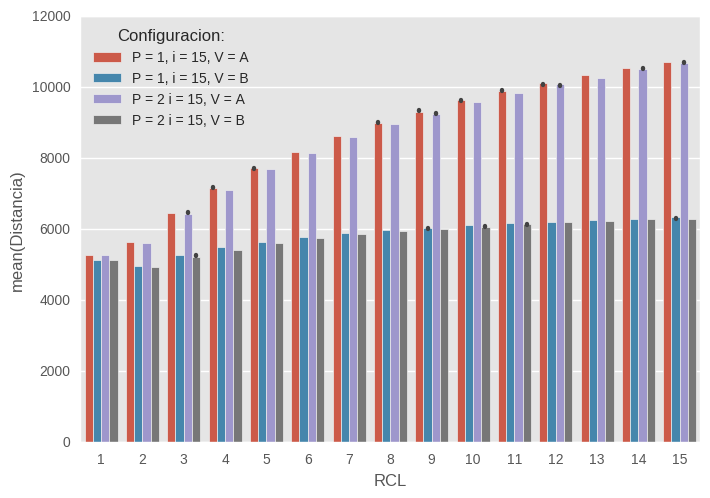
\includegraphics[width=0.7\columnwidth]{imagenes/Ej4/ej4_exp1_Distancia.png}
    \end{center}
\end{figure}


Para este entonces, volvemos a notar como el vecindario, es la sección fundamental de la metaheurística, dado que, comparando a partir de los vecindarios, el vecindario A es aquel que mejor distancia consigue, para todo criterio y para todo valor de RCL. La justificación de por qué las soluciones del vecindario A son mejores que las del vecindario B, está explicado en el \textbf{Ejercicio 3}. 
\par Para sacar una mejor conclusión, comparamos el vecindario A y el vecindario B independientemente. 
Por un lado, usando el vecindario A notamos que, para un RCL de tamaño 2 y para cualquier criterio, se consigue la mejor distancia. Esto podría deberse a que, a mayor RCL, las posibilidades de obtener una próxima estación con una distancia más corta, es menor, debido al factor random que obtiene una próxima estación de la RCL. Mientras que para un RCL de tamaño 1, el algoritmo metaheurístico pasaría a ser similar a un algoritmo greedy, junto con una búsqueda local, con lo cual recorrería menos soluciones. 
\par Por otro lado, dentro del vecindario A, no encontramos una mejora lo suficientemente notable como para decidir acerca de cuál criterio de parada es óptimo. 
\par También pudimos ver que con el vecindario B la calidad de solución empeora a medida que crece el RCL. Esto se debe a que cuanto más tamaño tenga RCL, en cada iteración donde se construye un recorrido, se elige una estación al azar entre las que entren dentro de la RCL. Cuanto más grande sea la RCL, más estaciones posibles serán las candidatas a ser la próxima a recorrer, y por lo tanto, mayor probabilidad habrá de que no se elija la óptima. 
También influye que en la búsqueda local, el vecindario B tiene una peor calidad de solución. 
\par También cabe destacar que, al igual que con el vecindario A, no notamos ninguna mejora a partir del criterio de parada. 
\par Luego de este experimento, concluímos que el algoritmo que utiliza el vecindario A, es quien devuelve una mejor solución, sin importar el criterio de parada. Y que al comparar en base al tamaño de la RCL, cuánto menor sea, mejor solución se va a obtener.


\par Finalmente, obtuvimos como conclusión de este experimento que, en principio, si se depende de la RCL, no se puede obtener un algoritmo eficiente en cuanto a tiempo y calidad de la solución a la vez. Por otro lado, pudimos comprender la fuerte influencia que tienen los vecindarios utilizados en la búsqueda local dentro del algoritmo, tanto para tiempos como para calidad de solución. Es decir, el vecindario A devolverá una mejor solución, en mayor tiempo, y el vecindario B, devolverá una peor solución, en menor tiempo. 
\par El tamaño de la RCL fue el segundo factor de crecimiento, tanto para distancia como para tiempos. En ambas comparaciones (exceptuando que en un RCL de tamaño 2, la solución mejoró), tanto el tiempo como la calidad de solución, empeoraban a medida que crecía. Luego, se buscará en próximos experimentos ver cuánto influye el criterio de parada y sus iteraciones.



\subsubsection{Experimento 2: Iterar el límite de los criterios de parada}

Para este experimento se usaron las mismas instancias que en el \textbf{Experimento 1}, pero esta vez en vez de fijar el criterio de parada e iterar el tamaño del RCL, se fijó el tamaño del RCL en la mitad de la cantidad de estaciones y se iteró de 1 a 15 el límite de ambos criterios de parada. De esta manera las 4 configuraciones son,


\begin{table}[H]
\centering
\begin{tabular}{ |c|c|c|c| } 
 \hline
 Instancias&Busqueda Local&Criterio de parada&RCL\\ 
 \hline
 Configuración 0 & Vecindario A & Iterar K veces & Estaciones/2\\
 \hline
 Configuración 1 & Vecindario A & Iterar hasta K peores & Estaciones/2\\
 \hline
 Configuración 2 & Vecindario B & Iterar K veces  & Estaciones/2\\
 \hline
 Configuración 3 & Vecindario B & Iterar hasta K peores & Estaciones/2\\
 \hline
\end{tabular}
\caption{Configuraciones experimento 2}
\end{table}

Luego, se corrió cada instancia 20 veces, y se calculó el promedio del tiempo y las distancias. 
Después por cada instancia cuyo vecindario de búsqueda local, criterio de parada y cantidad de iteraciones eran el mismo, se sacó el mismo promedio. Luego, por cada una de las 4 configuraciones, se obtuvieron 15 promedios de tiempo y distancia.



\begin{figure}[H]
    \begin{center}
      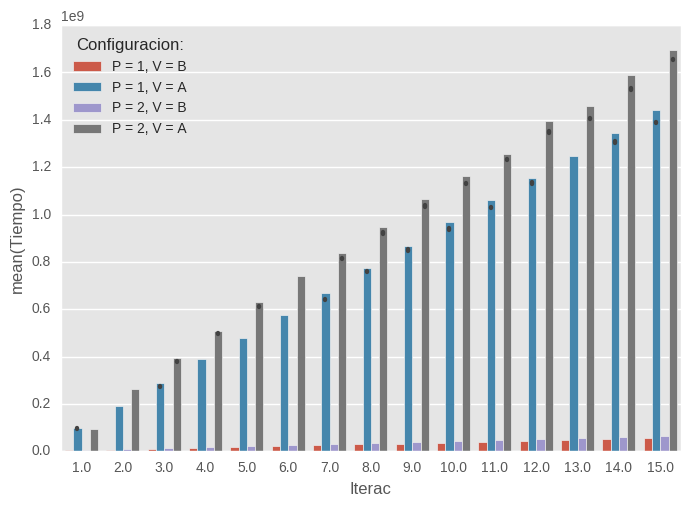
\includegraphics[width=0.7\columnwidth]{imagenes/Ej4/ej4_exp2_Tiempo.png}
    \end{center}
\end{figure}

Al igual que en el \textbf{Experimento 1}, la característica determinante de las instancias, que influye en el tiempo, es el vecindario utilizado en la búsqueda local. Luego, comparando cada vecindario en particular a medida que avanza la cantidad de iteraciones, en ambos criterios crece el tiempo de ejecución. Esto se debe claramente a que, a mayor cantidad de veces que se ejecuta un algoritmo, el tiempo de corrida crece. 
\par Luego, si se observa el vecindario A, hay una gran diferencia de tiempos entre cada criterio de parada del algoritmo. Para entender esto, se debe especificar en detalle cada criterio de parada. Es decir, esto se debe a que el \textbf{criterio 1} hace exactamente la cantidad de iteraciones que se le indique, mientras que el \textbf{criterio 2}, sea K la cantidad de iteraciones, se ejecuta hasta encontrar K soluciones peores. O sea, siendo i la cantidad de mejores soluciones que se encuentran, se harán K + i iteraciones, lo cual aumenta el tiempo de ejecución. Lo mismo se puede observar en el vecindario B. Aunque es mínima la diferencia de tiempos entre criterios, es el segundo factor que genera que tarde más, por el mismo motivo que en el vecindario A.
\par Como primer conclusión, si nos basamos en vecindarios de la búsqueda local, el vecindario que menos tiempo toma es el B. Y a la hora de elegir un criterio de parada, si se busca un menor tiempo, se debe hacer una sola iteración para cualquier criterio. Pero si es necesario iterar en alguno, se tomaría el \textbf{criterio 1}, donde la cantidad de iteraciones que se indique son las que se van a realizar.

\newpage
\par Luego para analizar la calidad de solución, 



\begin{figure}[H]
    \begin{center}
      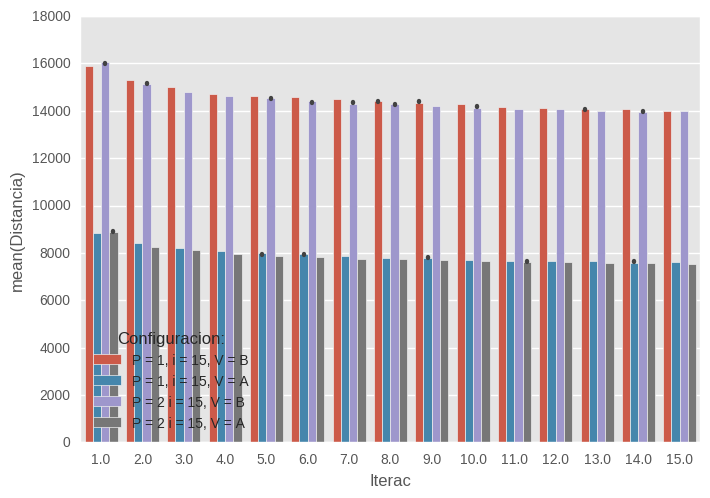
\includegraphics[width=0.7\columnwidth]{imagenes/Ej4/ej4_exp2_Distancia.png}
    \end{center}
\end{figure}



En primer lugar, el objetivo del criterio de parada es mejorar la solución. Cuantas más iteraciones se hace del algoritmo, mejor soluciones se encuentra. Es por esto que sin importar el vecindario ni el criterio, a mayor cantidad de iteraciones, mejores soluciones se encontrarán. 
\par Luego, el vecindario fue el factor que más influyó en el resultado, es decir, las soluciones del vecindario A son claramente mejores que las soluciones del vecindario B. Además, por cada vecindario, se observa que el criterio 1 está por debajo, en cuanto a calidad de solución, que el criterio 2. Esto se debe, como mencionamos anteriormente, a que si se itera K veces el \textbf{criterio 2}, cada vez que encuentra una mejor solución no se cuenta como iteración. Por lo tanto, sea i la cantidad de veces que se encontró una mejor solución, la cantidad de iteraciones será de  K+i. Al haber mayor cantidad de iteraciones, habrá mas probabilidad de mejorar la solución. Mientras que el \textbf{criterio 1} únicamente iterará K veces el algoritmo, sin importar la mejora de la solución.
\par De esta manera, concluímos que el criterio 2 es aquel que, a mayor cantidad de iteraciones, mejores soluciones encuentra (siempre y cuando esté complementado con el vecindario A de la búsqueda local).

\par Finalmente, como conclusión del segundo experimento, los resultados fueron similares al experimento 1. Debido a que si se busca una mejor solución, es necesario mayor tiempo de ejecución. Luego, si se busca una mejor solución, se debe usar el criterio de parada 2 iterando la mayor cantidad de veces posible, junto con el vecindario A. Mientras que si se busca una solución poco óptima en el menor tiempo posible, es necesario pocas iteraciones del criterio de parada 1, junto con el vecindario B. 


\subsubsection{Conclusión}

Luego de comparar cada configuración posible de la metaheurística, pudimos concluir que, uno de los principales problemas que se enfrentan para este tipo de algoritmo, es el criterio entre calidad de solución y tiempo de corrida. En ambos experimentos encontramos la misma problemática. Luego, si se busca optimizar más la solución, obtuvimos que es necesario elegir el vecindario A, junto con un RCL de tamaño 2, con el criterio de parada 2 haciendo la mayor cantidad de iteraciones posibles. Mientras que si se busca es un algoritmo metaheurístico rápido, es necesario el vecindario B, junto con un RCL de tamaño 1, con pocas iteraciones del criterio de parada 1.
\par Dado que una metaheurística tiene un factor aleatorio que influye en la calidad del resultado, si el algoritmo se ejecuta pocas veces, es difícil analizar la calidad del resultado. Sin embargo, al ejecutar el algoritmo una cantidad considerada de veces, es más probable que la calidad del resultado mejore. Pero como se sabe, cuantas más veces se ejecute el algoritmo, más alto va a ser el tiempo de ejecución.
\par Por lo tanto, creemos que antes de decidir la configuración de un algoritmo con una metaheurística, se debe analizar, y poner en una balanza, qué es más relevante: si obtener una mejor calidad de soluciones, o si obtener una solución lo antes posible.
\par Vale también destacar que creemos que la configuración de cuánto va a influir el factor aleatorio del algoritmo, se debe ir modificando y decidiendo en base a la calidad de resultados que se va obteniendo. Por ejemplo, si el tamaño de la RCL es de un único elemento (es decir, el algoritmo se asemeja al del Ejercicio 2) y la solución obtenida es mala comparada con la mejor solución que se podría obtener, se tiende a tomar la decisión de aumentar el tamaño de la RCL con la esperanza de obtener mejores soluciones.